% Template adapted from https://github.com/jgm/pandoc-templates/blob/master/default.latex
% To be used with XeLaTex in memoiR
%%%%%%%%%%%%%%%%%%%%%%%%%%%%%%%%%%%%%%%%%%%%%%%%%%%%%%%%%%%%%%%%%%%%%%%%%%%%%%%%%%%%%%%%%

% Options for packages loaded elsewhere
\PassOptionsToPackage{unicode=true}{hyperref}
\PassOptionsToPackage{hyphens}{url}
\PassOptionsToPackage{dvipsnames,svgnames*,x11names*}{xcolor}
% Right to left support


\documentclass[
  12pt,
  american,
  a4paper,
  extrafontsizes,onecolumn,openright
  ]{memoir}

% Double (or whatever) spacing

% Math
\usepackage{amssymb, amsmath}
% mathspec: arbitrary math fonts
\usepackage{unicode-math}
\defaultfontfeatures{Scale=MatchLowercase}
\defaultfontfeatures[\rmfamily]{Ligatures=TeX,Scale=1}

% Fonts
\usepackage{lmodern}
\usepackage{fontspec}
% Main font
% Specific sanserif font
% Specific monotype font
% Specific math font
% Chinese, Japanese, Corean fonts

% Use upquote for straight quotes in verbatim environments
\usepackage{upquote}
% Use microtype
\usepackage[]{microtype}
\UseMicrotypeSet[protrusion]{basicmath} % disable protrusion for tt fonts

% Verbatim in note

% Color links
\usepackage{xcolor}

% Strikeout

% Necessary for code chunks
\usepackage{color}
\usepackage{fancyvrb}
\newcommand{\VerbBar}{|}
\newcommand{\VERB}{\Verb[commandchars=\\\{\}]}
\DefineVerbatimEnvironment{Highlighting}{Verbatim}{commandchars=\\\{\}}
% Add ',fontsize=\small' for more characters per line
\usepackage{framed}
\definecolor{shadecolor}{RGB}{248,248,248}
\newenvironment{Shaded}{\begin{snugshade}}{\end{snugshade}}
\newcommand{\AlertTok}[1]{\textcolor[rgb]{0.94,0.16,0.16}{#1}}
\newcommand{\AnnotationTok}[1]{\textcolor[rgb]{0.56,0.35,0.01}{\textbf{\textit{#1}}}}
\newcommand{\AttributeTok}[1]{\textcolor[rgb]{0.77,0.63,0.00}{#1}}
\newcommand{\BaseNTok}[1]{\textcolor[rgb]{0.00,0.00,0.81}{#1}}
\newcommand{\BuiltInTok}[1]{#1}
\newcommand{\CharTok}[1]{\textcolor[rgb]{0.31,0.60,0.02}{#1}}
\newcommand{\CommentTok}[1]{\textcolor[rgb]{0.56,0.35,0.01}{\textit{#1}}}
\newcommand{\CommentVarTok}[1]{\textcolor[rgb]{0.56,0.35,0.01}{\textbf{\textit{#1}}}}
\newcommand{\ConstantTok}[1]{\textcolor[rgb]{0.00,0.00,0.00}{#1}}
\newcommand{\ControlFlowTok}[1]{\textcolor[rgb]{0.13,0.29,0.53}{\textbf{#1}}}
\newcommand{\DataTypeTok}[1]{\textcolor[rgb]{0.13,0.29,0.53}{#1}}
\newcommand{\DecValTok}[1]{\textcolor[rgb]{0.00,0.00,0.81}{#1}}
\newcommand{\DocumentationTok}[1]{\textcolor[rgb]{0.56,0.35,0.01}{\textbf{\textit{#1}}}}
\newcommand{\ErrorTok}[1]{\textcolor[rgb]{0.64,0.00,0.00}{\textbf{#1}}}
\newcommand{\ExtensionTok}[1]{#1}
\newcommand{\FloatTok}[1]{\textcolor[rgb]{0.00,0.00,0.81}{#1}}
\newcommand{\FunctionTok}[1]{\textcolor[rgb]{0.00,0.00,0.00}{#1}}
\newcommand{\ImportTok}[1]{#1}
\newcommand{\InformationTok}[1]{\textcolor[rgb]{0.56,0.35,0.01}{\textbf{\textit{#1}}}}
\newcommand{\KeywordTok}[1]{\textcolor[rgb]{0.13,0.29,0.53}{\textbf{#1}}}
\newcommand{\NormalTok}[1]{#1}
\newcommand{\OperatorTok}[1]{\textcolor[rgb]{0.81,0.36,0.00}{\textbf{#1}}}
\newcommand{\OtherTok}[1]{\textcolor[rgb]{0.56,0.35,0.01}{#1}}
\newcommand{\PreprocessorTok}[1]{\textcolor[rgb]{0.56,0.35,0.01}{\textit{#1}}}
\newcommand{\RegionMarkerTok}[1]{#1}
\newcommand{\SpecialCharTok}[1]{\textcolor[rgb]{0.00,0.00,0.00}{#1}}
\newcommand{\SpecialStringTok}[1]{\textcolor[rgb]{0.31,0.60,0.02}{#1}}
\newcommand{\StringTok}[1]{\textcolor[rgb]{0.31,0.60,0.02}{#1}}
\newcommand{\VariableTok}[1]{\textcolor[rgb]{0.00,0.00,0.00}{#1}}
\newcommand{\VerbatimStringTok}[1]{\textcolor[rgb]{0.31,0.60,0.02}{#1}}
\newcommand{\WarningTok}[1]{\textcolor[rgb]{0.56,0.35,0.01}{\textbf{\textit{#1}}}}

% Listings package

% Tables
\usepackage{longtable,booktabs,tabu}
% Fix footnotes in tables (requires footnote package)
\IfFileExists{footnote.sty}{\usepackage{footnote}\makesavenoteenv{longtable}}{}

% Graphics
\usepackage{graphicx,grffile}
\graphicspath{{images/}}
\makeatletter
\def\maxwidth{\ifdim\Gin@nat@width>\linewidth\linewidth\else\Gin@nat@width\fi}
\def\maxheight{\ifdim\Gin@nat@height>\textheight\textheight\else\Gin@nat@height\fi}
\makeatother
% Scale images if necessary, so that they will not overflow the page
% margins by default, and it is still possible to overwrite the defaults
% using explicit options in \includegraphics[width, height, ...]{}
\setkeys{Gin}{width=\maxwidth,height=\maxheight,keepaspectratio}

% Prevent overfull lines
\setlength{\emergencystretch}{3em}  
\providecommand{\tightlist}{%
  \setlength{\itemsep}{0pt}\setlength{\parskip}{0pt}}

% Number sections for memoir (secnumdepth counter is ignored)
\setsecnumdepth{section}

% Set default figure placement to htbp
\makeatletter
\def\fps@figure{htbp}
\makeatother

% Spacing in lists
\usepackage{enumitem}

% Polyglossia
\usepackage{polyglossia}
\setmainlanguage{en-US}
\setotherlanguage{fr-FR}
\setotherlanguage{it}

% BibLaTeX
\usepackage[backend=biber,style=authoryear-ibid,isbn=false,backref=true,giveninits=true,uniquename=init,maxcitenames=2,maxbibnames=150,sorting=nyt,sortcites=false]{biblatex}
\addbibresource{references.bib}

% cslreferences environment required by pandoc > 2.7



%%%%%%%%%%%%%%%%%%%%%%%%%%%%%%%%%%%%%%%%%%%%%%%%%%%%%%%%%%
% memoiR format

% Chapter Summary environment 
\usepackage[tikz]{bclogo}
\newenvironment{Summary}
  {\begin{bclogo}[logo=\bctrombone, noborder=true, couleur=lightgray!50]{In a Nutshell}\parindent0pt}
  {\end{bclogo}}
% Syntax:
%
%```{block, type='Summary'}
% Deliver message here.
% ```

% scriptsize code 
\let\oldverbatim\verbatim
\def\verbatim{\oldverbatim\scriptsize}
% Applies to code blocks and R code results
% code chunk options size='scriptsize' applies only to R code and results
% if the code chunk sets a different size, \def\verbatim{...} is prioritary for code results 


% Layout
%%%%%%%%%%%%%%%%%%%%%%%%%%%%%%%%%%%%%%%%%%%%%%%%%%%%%%%%%%

% Based on memoir, style companion
\newcommand{\MemoirChapStyle}{daleif1}
\newcommand{\MemoirPageStyle}{Ruled}

% Space between paragraphs
\usepackage{parskip}
  \abnormalparskip{3pt}

% Adjust margin paragraphs vertical position
\usepackage{marginfix}


% Margins
%%%%%%%%%%%%%%%%%%%%%%%%%%%%%%%%%%%%%%%

% allow use of '-',+','/' ans '*' to make simple length computation
\usepackage{calc}

% Full-width figures utilities
\newlength\widthw % full width
\newlength{\rf}
\newcommand*{\definesHSpace}{
  \strictpagecheck % slower but efficient detection of odd/even pages
  \checkoddpage
  \ifoddpage
  \setlength{\rf}{0mm}
  \else
  \setlength{\rf}{\marginparsep+\marginparwidth}
  \fi
}

\makeatletter
% 1" margins for the front matter.
\newcommand*{\SmallMargins}{
  \setlrmarginsandblock{1.5in}{1.5in}{*}
  \setmarginnotes{0.1in}{0.1in}{0.1in}
 \setulmarginsandblock{1.5in}{1in}{*}
  \checkandfixthelayout
  \ch@ngetext
  \clearpage
  \setlength{\widthw}{\textwidth+\marginparsep+\marginparwidth}
  \footnotesatfoot
  \chapterstyle{\MemoirChapStyle}  % Chapter and page styles must be recalled
  \pagestyle{\MemoirPageStyle}
}

% 3" outer margin for the main matter
\newcommand{\LargeMargins}{\SmallMargins}
\makeatother

% Figure captions and footnotes in outer margins


% Main title page with filigrane
%%%%%%%%%%%%%%%%%%%%%%%%%%%%%%%%%%%%%%%%%%%%%%%%%%%%%%%%%%

% Text blocks
\usepackage[absolute,overlay]{textpos}
  \setlength{\TPHorizModule}{1mm}
  \setlength{\TPVertModule}{1mm}

\newcommand{\MainTitlePage}[2]{
  \SmallMargins % Margins
  \pagestyle{empty} % No header/footer
  \textblockorigin{\stockwidth-\paperwidth-\trimedge}{\trimtop} % recto
  \begin{textblock*}{2mm}(\spinemargin/2,\uppermargin/2)
    \rule{1pt}{\paperheight-\uppermargin}
  \end{textblock*}
  \begin{textblock*}{\paperwidth*2/3}(\paperwidth/5, \paperheight/5)
    \flushright
    \begin{Spacing}{3}
      {\fontfamily{qtm}\selectfont\fontsize{45}{45}\selectfont\textsc{\thetitle}}
    \end{Spacing}
  \end{textblock*}
    \begin{textblock*}{\paperwidth*2/3}(\paperwidth/5, \paperheight/2)
    \flushright
    {\fontfamily{qtm}\huge\theauthor}
  \end{textblock*}
    \begin{textblock*}{\paperwidth*2/3}[0, 1](\spinemargin, \uppermargin+\textheight)
    \normalfont\thedate
  \end{textblock*}
  ~\\ % Print a character or the page will not exist
  \newpage
  \textblockorigin{\trimedge}{\trimtop} % verso
  \begin{textblock*}{\textwidth}(\paperwidth-\spinemargin-\textwidth, \uppermargin)
    #1
  \end{textblock*}
  \begin{textblock*}{\textwidth}[0,1](\paperwidth-\spinemargin-\textwidth, \uppermargin+\textheight+\footskip)
    \centering
    
\includegraphics[width=\paperwidth/4]{logo}\\ \bigskip
    #2
  \end{textblock*}
  ~\\ % Print a character or the page will not exist
  \newpage
}

% Clear page and open an even one (\clearpage opens an odd one)
\newcommand{\evenpage}{
  \clearpage
  \strictpagecheck % slower but efficient detection of odd/even pages
  \checkoddpage
  \ifoddpage
    \thispagestyle{empty}
    ~\\ % Print a character or the page will not exist
    \newpage
  \else
    % do nothing
  \fi
}


%% PDF title page to insert
%%%%%%%%%%%%%%%%%%%%%%%%%%%%%%%%%%%%%%%%%%%%%%%%%%%%%%%%%%

\usepackage{pdfpages}


%% Bibliography
%%%%%%%%%%%%%%%%%%%%%%%%%%%%%%%%%%%%%%%%%%%%%%%%%%%%%%%%%%

\usepackage[strict,autostyle]{csquotes}
% Repeated citation as author-year-title instead of author-title (modification of footcite:note in verbose-inote.cbx)

%% Table of Contents
%%%%%%%%%%%%%%%%%%%%%%%%%%%%%%%%%%%%%%%%%%%%%%%%%%%%%%%%%%

% fix the typesetting of the part number
\renewcommand\partnumberlinebox[2]{#2\ ---\ }


% Fonts
%%%%%%%%%%%%%%%%%%%%%%%%%%%%%%%%%%%%%%%%%%%%%%%%%%%%%%%%%%


% Hyperref comes last
%%%%%%%%%%%%%%%%%%%%%%%%%%%%%%%%%%%%%%%%%%%%%%%%%%%%%%%%%%

\usepackage{hyperref}
\hypersetup{
  pdftitle={Memoir Template},
  pdfauthor={Marion Boisseaux, Tristan Lafont Rapnouil and hopefully many other people},
  colorlinks=true,
  linkcolor=Maroon,
  citecolor=Blue,
  urlcolor=Blue,
  breaklinks=true}

% Don't use monospace font for urls
\urlstyle{same}


% Title, author, date from YAML to LaTeX
%%%%%%%%%%%%%%%%%%%%%%%%%%%%%%%%%%%%%%%%%%%%%%%%%%%%%%%%%%

\title{Memoir Template}

\author{Marion Boisseaux, Tristan Lafont Rapnouil and hopefully many other people}

\date{2023-02-17}


% Include headers (preamble.tex) here
%%%%%%%%%%%%%%%%%%%%%%%%%%%%%%%%%%%%%%%%%%%%%%%%%%%%%%%%%%
% Add LaTeX code into the preamble of the document here
\hyphenation{bio-di-ver-si-ty sap-lings}


%%%%%%%%%%%%%%%%%%%%%%%%%%%%%%%%%%%%%%%%%%%%%%%%%%%%%%%%%%%%%%%%%%%%%%%%%
% memoiR dalef3 chapter style 
% https://ctan.crest.fr/tex-archive/info/latex-samples/MemoirChapStyles/MemoirChapStyles.pdf
\usepackage{soul}
\definecolor{nicered}{rgb}{.647,.129,.149}
\makeatletter
\newlength\dlf@normtxtw
\setlength\dlf@normtxtw{\textwidth}
\def\myhelvetfont{\def\sfdefault{mdput}}
\newsavebox{\feline@chapter}
\newcommand\feline@chapter@marker[1][4cm]{%
  \sbox\feline@chapter{%
    \resizebox{!}{#1}{\fboxsep=1pt%
	  \colorbox{nicered}{\color{white}\bfseries\sffamily\thechapter}%
	}}%
  \rotatebox{90}{%
    \resizebox{%
	  \heightof{\usebox{\feline@chapter}}+\depthof{\usebox{\feline@chapter}}}%
	{!}{\scshape\so\@chapapp}}\quad%
  \raisebox{\depthof{\usebox{\feline@chapter}}}{\usebox{\feline@chapter}}%
 }
\newcommand\feline@chm[1][4cm]{%
  \sbox\feline@chapter{\feline@chapter@marker[#1]}%
  \makebox[0pt][l]{% aka \rlap
    \makebox[1cm][r]{\usebox\feline@chapter}%
  }}
\makechapterstyle{daleif1}{
  \renewcommand\chapnamefont{\normalfont\Large\scshape\raggedleft\so}
  \renewcommand\chaptitlefont{\normalfont\huge\bfseries\scshape\color{nicered}}
  \renewcommand\chapternamenum{}
  \renewcommand\printchaptername{}
  \renewcommand\printchapternum{\null\hfill\feline@chm[2.5cm]\par}
  \renewcommand\afterchapternum{\par\vskip\midchapskip}
  \renewcommand\printchaptertitle[1]{\chaptitlefont\raggedleft ##1\par}
}
\makeatother
\usepackage{booktabs}
\usepackage{longtable}
\usepackage{array}
\usepackage{multirow}
\usepackage{wrapfig}
\usepackage{float}
\usepackage{colortbl}
\usepackage{pdflscape}
\usepackage{tabu}
\usepackage{threeparttable}
\usepackage{threeparttablex}
\usepackage[normalem]{ulem}
\usepackage{makecell}
\usepackage{xcolor}


% End of preamble
%%%%%%%%%%%%%%%%%%%%%%%%%%%%%%%%%%%%%%%%%%%%%%%%%%%%%%%%%%


\begin{document}
\frontmatter

% Title page
%%%%%%%%%%%%%%%%%%%%%%%%%%%%%%%%%%%%%%%%%%%%%%%%%%%%%%%%%%

\includepdf[pages=1]{images/mariono.pdf}
\cleardoublepage

\MainTitlePage{This document is reproducible thanks to:

\begin{itemize}
  \item \LaTeX and its class memoir (\url{http://www.ctan.org/pkg/memoir}).
  \item R (\url{http://www.r-project.org/}) and RStudio (\url{http://www.rstudio.com/})
  \item bookdown (\url{http://bookdown.org/}) and memoiR (\url{https://ericmarcon.github.io/memoiR/})
\end{itemize}}{Name of the owner of the logo

\url{http://www.company.com}

An explanatory sentence.
Leave an empty line for line breaks.}


% Before Body
%%%%%%%%%%%%%%%%%%%%%%%%%%%%%%%%%%%%%%%%%%%%%%%%%%%%%%%%%%





% Contents
%%%%%%%%%%%%%%%%%%%%%%%%%%%%%%%%%%%%%%%%%%%%%%%%%%%%%%%%%%

\LargeMargins
{
\hypersetup{linkcolor=}
\setcounter{tocdepth}{2}
\tableofcontents
}


% Body
%%%%%%%%%%%%%%%%%%%%%%%%%%%%%%%%%%%%%%%%%%%%%%%%%%%%%%%%%%

\LargeMargins
\hypertarget{intro}{%
\chapter{Introduction}\label{intro}}

Plant functional traits are the features (morphological, physiological, phenological) that represent ecological strategies and determine \emph{describe?} how plants respond to environmental factors, affect other trophic levels and influence ecosystem properties.
Variation in plant functional traits, and trait syndromes, has proven useful for tackling many important ecological questions at a range of scales, giving rise to a demand for standardized ways to measure ecologically meaningful plant traits.
The importance of these topics dictates the urgent need for more and better data, and increases the value of standardized protocols for quantifying trait variation of different species, in particular for traits with power to predict plant- and ecosystem-level processes, and for traits that can be measured relatively easily (Pérez-Harguindeguy et al., 2013)

This handbook presents the different protocols used in EcoFoG's ecophysio lab.
We therefore suggest the methodological principles for a more open and transparent science.
This handbook not only includes updated methods for the trait measurements, but also includes the excel worksheets for data collection and links toward detailed tutorial or user's guide for all methods used in this lab.
This handbook will be associated with an R package \protect\hyperlink{ecophycofog-package}{EcophyCofog} containing some useful homemade functions to deal with some devices output.

\mainmatter

\hypertarget{handbook-architecture}{%
\chapter{Handbook architecture}\label{handbook-architecture}}

This handbook is written for operational ends. As such, it is not a review or scientific paper thoroughly presenting each traits but rather a list of protocols associated with routinely measured traits in this lab.

Each chapter of this book correspond to one trait and associated measurement process.

\protect\hyperlink{morpho-anatomy}{Morpho-anatomy}

\protect\hyperlink{hydraulics}{Hydraulics}

\protect\hyperlink{fluorescence}{Fluorescence}

\protect\hyperlink{gaz-fluxes-and-exchanges}{Gaz fluxes and exchanges}

\protect\hyperlink{ecophycofog-package}{EcophyCofog Package}

\protect\hyperlink{greenhouse-setups-and-tips}{Greenhouse setups and tips}

\protect\hyperlink{device-info}{Device info}

\hypertarget{morpho-anatomy}{%
\chapter{Morpho-anatomy}\label{morpho-anatomy}}

\hypertarget{shoot-traits}{%
\section{Shoot traits}\label{shoot-traits}}

Shoot traits refer to all morpho-anatomical traits that can be measured on plant aerial part.
Most of these traits are measured on the leaves but see \protect\hyperlink{stem}{Stem} section.

\hypertarget{mass-associated-traits}{%
\subsection{Mass associated traits}\label{mass-associated-traits}}

Plant growth strategies and overall performances are often assessed via mass associated traits.
Three masses are used to calculate different metrics.
The \emph{Fresh Mass} (\textbf{FM}) which is the weight of freshly sampled leaves.
The \emph{Turgid Mass} (\textbf{TM}) which is the mass of fully hydrated leaves.
Leaf hydratation protocols are source of debate in EcoFog but are presented {[}here{]}{[}Leaf hydratation{]}
And the \emph{Dry Mass} (\textbf{DM}) which is the mass of dryed leaves.

To be compared, these weights must come from the same sample and we must measure the leaf projected surfaces.
See \protect\hyperlink{leaf-surface}{here} for the leaf surface measurements protocols.

From these masses and surfaces are calculated metrics such as SLA/LMA, RWC, LDMC, WHC (\protect\hyperlink{calculation}{Calculation}).

\textcolor{red}{Use the same balance for all you masses within an experiment!!}

\hypertarget{leaf-surface}{%
\subsubsection{Leaf surface}\label{leaf-surface}}

Most of leaf surfaces are obtained from leaf scans using office scanner.
The used scanners are \href{document/machine/EPSON_V800/usersguide.pdf}{EPSON's V800}.
To acquire leaf scans please see \protect\hyperlink{image-acquisition}{Image Acquisition}.
Depending on your research question you can either scan one leaf or several leaves (to have total leaf surface of your plant for instance).

Once you have one scan per experimental unit you need to extract its surface.
Surface measurements are made with the \href{document/software/ImageJ/user-guide-A4booklet.pdf}{\texttt{ImageJ}} freeware.
\texttt{ImageJ} works on all \texttt{OS} and can be downloaded {[}here{]}{[}\url{https://imagej.nih.gov/ij/download.html}{]}

Surface can be measured \textbf{manually} or \textbf{automatically}

\textbf{Manual measurements} :

Launch imageJ -\textgreater{} File -\textgreater{} Open (Ctrl + O) and browse for the picture you want to analyse.

Then select the \texttt{polygon\ selection} tool \ref{fig:polygon}.

\scriptsize

\begin{figure}

{\centering 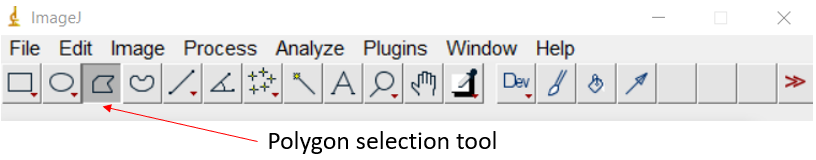
\includegraphics[width=0.5\linewidth]{document/trait/shootmorpho/polygon_selection_imageJ} 

}

\caption{Polygon selection tool in ImageJ}\label{fig:polygon}
\end{figure}

\normalsize

Zoom (\texttt{-}/\texttt{+} or \texttt{Ctrl+wheel\ in/out}) into your image to see only the leaf you want to measure \ref{fig:zoomin}.

\scriptsize

\begin{figure}

{\centering \includegraphics[width=0.5\linewidth]{document/trait/shootmorpho/Zoomin} 

}

\caption{Zooming in ImageJ}\label{fig:zoomin}
\end{figure}

\normalsize

Then you can \texttt{left\ click} to detour your leaf \ref{fig:detouring}.
The more points you have the more precise and close to the leaf your measruments will be.
However, bear in mind that this is laborious and that as your zoomed in your error should be negligeable.

\scriptsize

\begin{figure}

{\centering 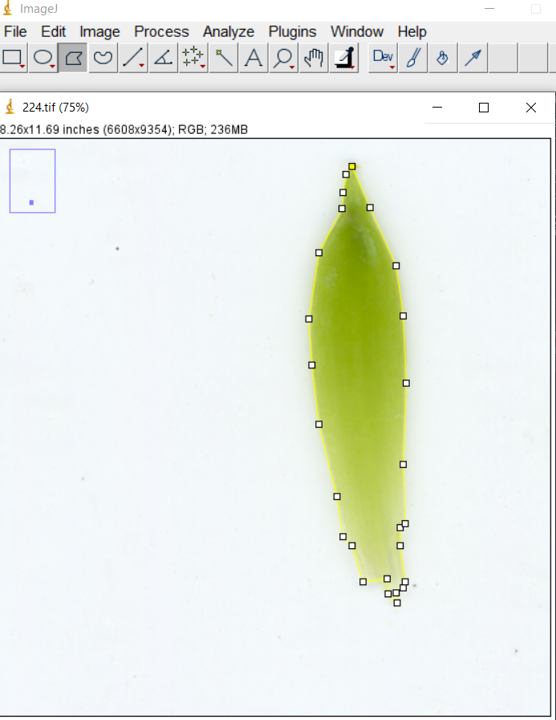
\includegraphics[width=0.5\linewidth]{document/trait/shootmorpho/detouring_leaf} 

}

\caption{Leaf detouring in ImageJ}\label{fig:detouring}
\end{figure}

\normalsize

Once you've closed your polygon, press \texttt{ctrl+M}.
A window containing the results will pop-up \ref{fig:ctrlmpopup}.

\scriptsize

\begin{figure}

{\centering 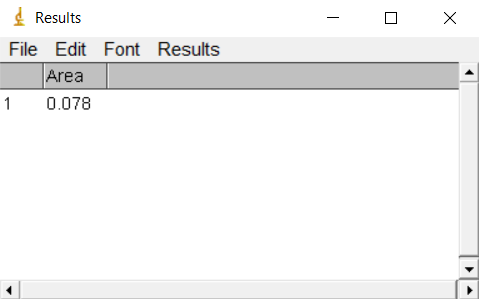
\includegraphics[width=0.5\linewidth]{document/trait/shootmorpho/ctrlMpopup} 

}

\caption{Results window in ImageJ}\label{fig:ctrlmpopup}
\end{figure}

\normalsize

The Area will be expressed in the units of your photo.
Some pictures have embedded scales in cm or inches but the default is usually in pixels (px).
For more information see {[}ImageJ scale{]}.

Each measurements will be added to the results window (one each time you press \texttt{ctrl+M}).
You can then save this window in the \texttt{.csv}format clicking on \texttt{File}, \texttt{Save\ As} and browse for chosen location.
You can either have one file per photo (i.e.~sample) and then name your file as your sample ID.
Or you can decide to have one file for all your samples.
Then you have to remember or write somewhere which measurements ID is associated to each of your samples to find who's who \ref{fig:measid}.

\scriptsize

\begin{figure}

{\centering 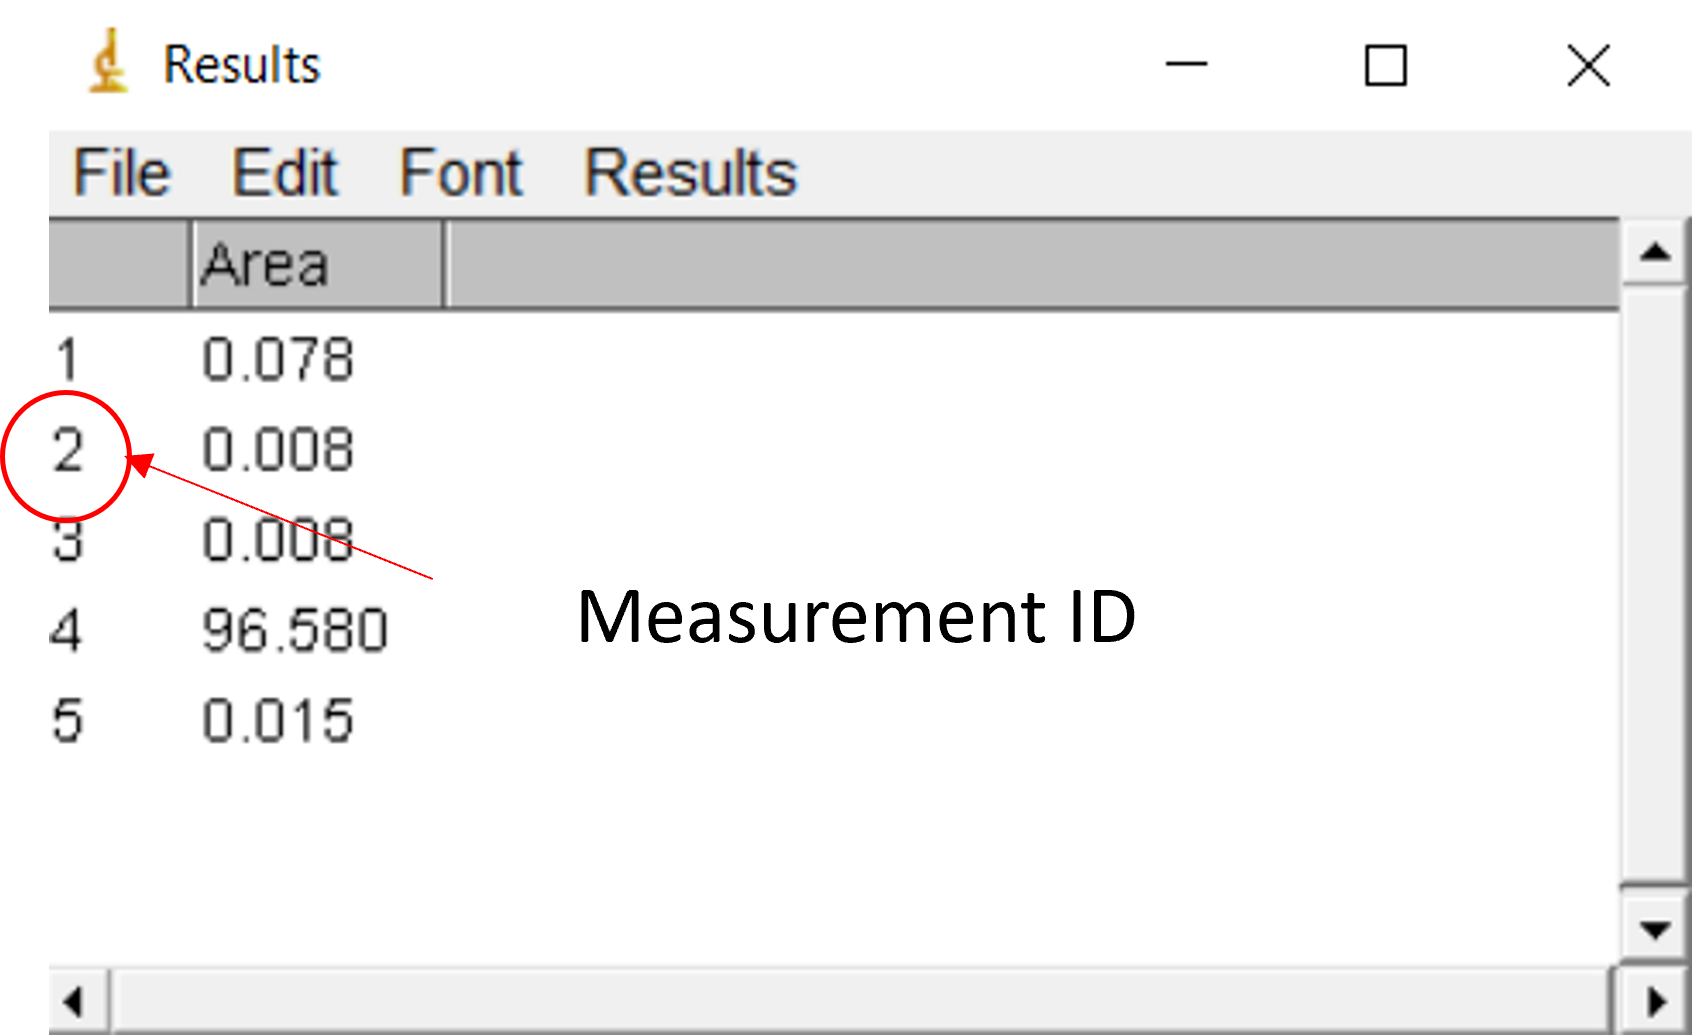
\includegraphics[width=0.5\linewidth]{document/trait/shootmorpho/measurementID} 

}

\caption{Measurement ID in ImageJ}\label{fig:measid}
\end{figure}

\normalsize

\textbf{Automatic measurements}:

This will allow you to analyze many data at the same time.
To do so you will need to use an homemade ImageJ macro.

\href{document/software/ImageJ/macro.txt}{Macro exemple}.
This macro is used to convert your colored scans in 8 bit black and white pictures.
Then it set scale for 800 ppi scans (distances=800px known = 2.54 cm , pixel = 1).
With ppi -\textgreater{} pixel per inch and 1 inch = 2.54cm.
The pixel ratio is 1 as vertical and horizontal resolution is the same.
It sets the contrast and then anaylze size of particle bigger than 0.01 cm\^{}2 and smaller than infinity.
It displays the results in summarize form for each pictures in the folder.

See \href{https://exeter-data-analytics.github.io/imagej-gui/macros.html}{here} for a tutorial on macro recording in imageJ.

To launch a batch process go to \texttt{Process}-\textgreater{} \texttt{Batch}-\textgreater{} \texttt{Macro...}.
This will open a window.
Fill the fields as follow:
+ \texttt{Input}: folder containing your pictures to be annalyzed
+ \texttt{Output}: folder to receive your output.
+ \texttt{Output\ format}: quite clear!

\hypertarget{calculation}{%
\subsubsection{Calculation}\label{calculation}}

\scriptsize

\begin{table}

\caption{\label{tab:unnamed-chunk-1}Mass derived traits}
\centering
\begin{tabular}[t]{lll}
\toprule
Acronym & Full name & Formula\\
\midrule
LA & Leaf area & \\
FM & Fresh mass & \\
TM & Turgid mass & \\
DM & Dry mass & \\
LMA & Leaf mass area & $DM/LA$\\
\addlinespace
SLA & Specific leaf area & $LA/DM$\\
LDMC & Leaf dry mass content & $DM/FM$\\
LS & Leaf succulence & $(FM-DM)/LA$\\
RWC & Relative water content & $[(FM-DM)/(TM-DM)]*100$\\
WHC & Water holding capcity & $(TM-DM)/LA$\\
\bottomrule
\end{tabular}
\end{table}

\normalsize

\hypertarget{leaf-anatomy}{%
\subsection{Leaf anatomy}\label{leaf-anatomy}}

\hypertarget{stomata-and-trichomes-density}{%
\subsubsection{Stomata and trichomes density}\label{stomata-and-trichomes-density}}

Stomata and trichomes density are acquired via epidermis printing.
First, apply double sided tape on your leaf and remove it.
You now have a piece of tape with your trichomes on it.
Place it on a glass-slide with the trichome-covered side on the top.

Then, to get your stomata, apply a thin coat of transparent nail polish and let it to dry.
Then you remove it with double-sided tape and put it on a glass slide (nail polish on top).

Observations are made with the \href{document/machine/Olympus\%20BX51/olympus_bx-51_bx52_microscope_manual.pdf}{\texttt{Olympus\ BX51}} microscope.

And pictures are taken with the installed camera (currently \href{document/machine/Lumenera\%20LW1135C-IO/Lumenera-USB-GigE-Camera-User-Manual.pdf}{\texttt{Lumenera\ LW1135C-IO}} but about to change).

Pictures can then be uploaded in ImageJ and you can manually count stomata and trichomes using the \texttt{multipoint} tool.

\textbf{There is a new opportunity to use \texttt{LabelStoma}, a deep leaning software for stomata detection.
It is developed by Ángela Casado-García and we are trying to make it work on some species that we study at EcoFog.}

\hypertarget{anatomical-structure}{%
\subsubsection{Anatomical structure}\label{anatomical-structure}}

Leaf anatomical observations are made on razor blade hand-made cross sections of leaves.

\scriptsize

\begin{figure}

{\centering 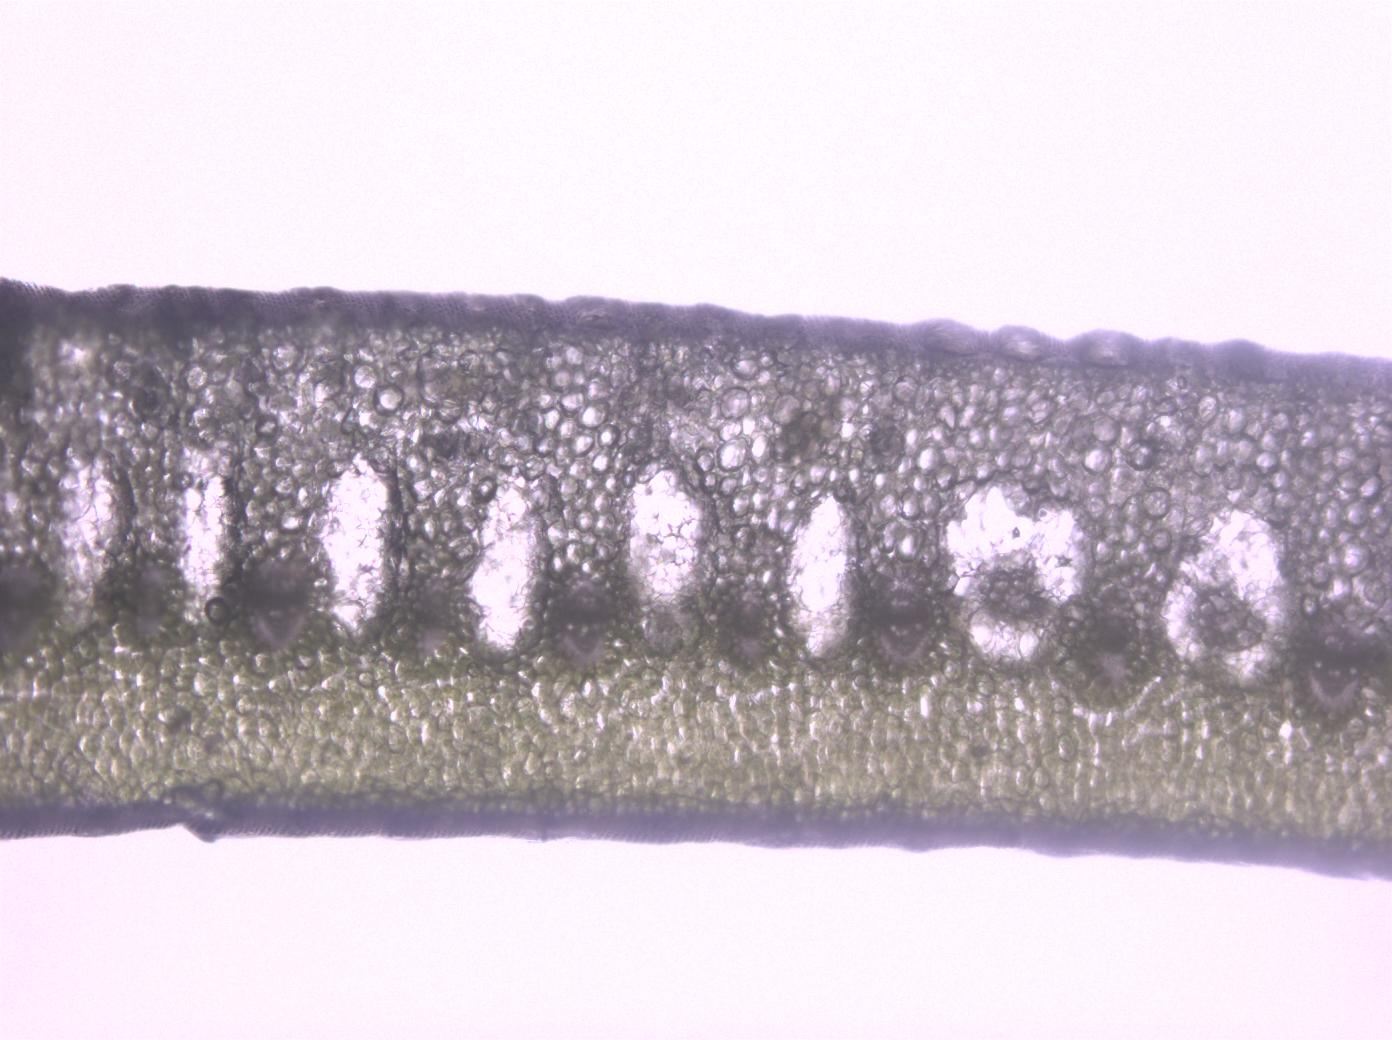
\includegraphics[width=0.5\linewidth]{document/trait/shootmorpho/bromecut1} 

}

\caption{Hand made cross section of a bromeliad leaf}\label{fig:bromecut}
\end{figure}

\normalsize

These cuts are directly placed in water/oil on a glass-slide and observed with the \href{document/machine/Olympus\%20BX51/olympus_bx-51_bx52_microscope_manual.pdf}{\texttt{Olympus\ BX51}} microscope.

And pictures are taken with the installed camera (currently \href{document/machine/Lumenera\%20LW1135C-IO/Lumenera-USB-GigE-Camera-User-Manual.pdf}{\texttt{Lumenera\ LW1135C-IO}} but about to change).

\textcolor{red}{Always use the same picture format!!}
We recommend \texttt{JPEG} or \texttt{TIFF}.

On these pictures you can then make measurements such as width of the epidermis and cuticle.
The width of certain type of tissue (chlorenchyma, parenchyma, hydrenchyma) or the distance between vessels using ImageJ tools such as the \texttt{draw\ segment} and \texttt{ctrl+M} output (area, angle of the line and length).

\scriptsize

\begin{figure}

{\centering 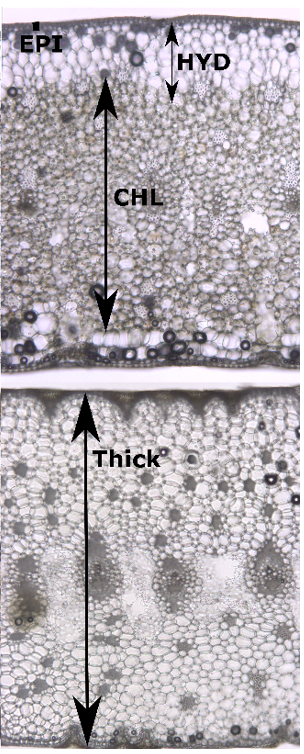
\includegraphics[width=0.5\linewidth]{document/trait/shootmorpho/meas_anat_tissue} 

}

\caption{Hand made cross section of a bromeliad leaf and possible anatomical measurements}\label{fig:measurements}
\end{figure}

\normalsize

\hypertarget{stem}{%
\subsection{Stem}\label{stem}}

\hypertarget{root-traits}{%
\section{Root traits}\label{root-traits}}

Root morphology analysis (length, diameter, etc.) are conducted using the Winrhizo software.

Winrhizo is a licenced software created by Regent Instrument Canada Inc.~It exist 4 different version and we own the \emph{Basic Version}. It allows root morphology analysis from scans.

\hypertarget{image-acquisition}{%
\subsection{Image Acquisition}\label{image-acquisition}}

\hypertarget{format}{%
\subsubsection{Format}\label{format}}

Supported image format are \texttt{.TIFF}, \texttt{.JPEG} and \texttt{.BMP}. \texttt{.TIFF}and \texttt{.BMP} are not compressed and are thus to be preferred. \texttt{.TIFF} images are compatible with all OS and should be privileged but you must be careful to save them \emph{uncompressed} as \texttt{WinRhizo} won't be able to open \emph{compressed} ones.

The higher the resolution, the more pixel you will have and the more precise will be your measurements. However, with resolution, scan time and image size increase. 800DPI is the standard in this lab but 400 is the winrhizo recommendation. This depend on the required level of precision as well as the size of the analyzed roots ( the finer the higher must be the resolution to get more details).

\hypertarget{scanner}{%
\subsubsection{Scanner}\label{scanner}}

Any scanner can be used to acquire scans for Winrhizo software. However, be sure that the format is compatible and that all the images inside your project are saved in the same format and the same resolution. For coherence purposes we encourage you to use the same formats between studies at Ecofog's lab scale.
\href{document/machine/EPSON_V800/usersguide.pdf}{EPSON's V800} scanners are the ones used as this document is being written. The scanner model isn't important but we recommend to use scanners with a transparent (double-lamp) option. This will allow cleaner root scans for complex root systems.
And the scanning software is \href{https://www.hamrick.com/vuescan/epson.html}{VueScan}

\hypertarget{scan-process}{%
\subsubsection{Scan process}\label{scan-process}}

\href{document/trait/rootmorpho/Parametre_Scanner.pdf}{protocol}

\hypertarget{flat-scan}{%
\paragraph{Flat scan}\label{flat-scan}}

You can decide to use basic scan options with light only coming from below. If you do so you need to have a white background installed under the scanner's roof (if black roots, if pale ones you'll need a black background).

Choosing this option will simplify your protocol and can suffice for simple and thin enough root systems.

\textbf{EXEMPLE} scan marion

\hypertarget{transparent}{%
\paragraph{Transparent}\label{transparent}}

If your root are too big \ref{fig:bigroots}, then self-shading can appear on flat scan and bias winrhizo's analysis. To avoid this shading you can remove the background from the scanner's roof to enable double-lamp scanning. The light coming from top and bottom as one, shading will be avoid and scans will be cleaner.

\scriptsize

\begin{figure}

{\centering 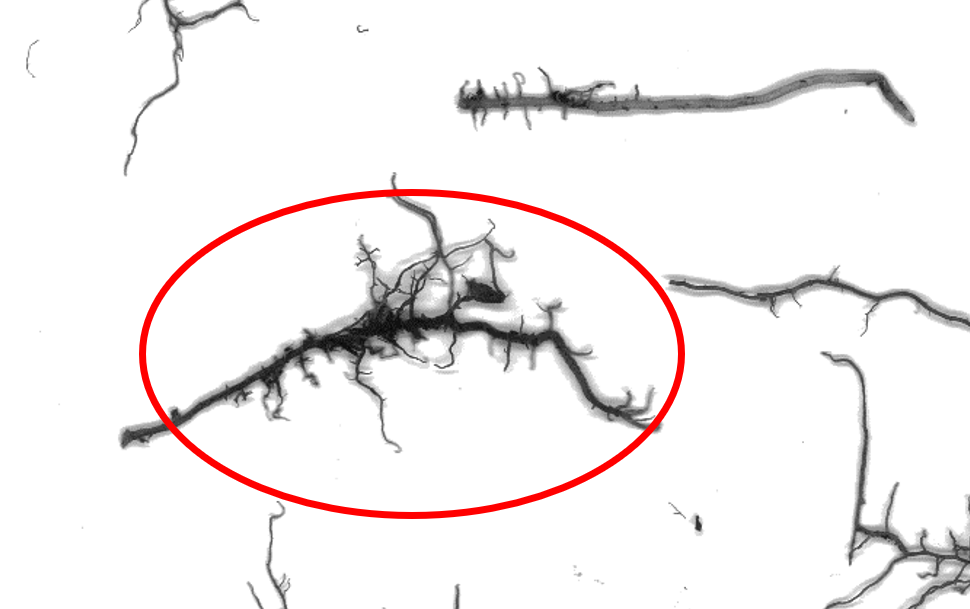
\includegraphics[width=0.5\linewidth]{document/trait/rootmorpho/thickroot} 

}

\caption{Roots to thick to be flat scanned}\label{fig:bigroots}
\end{figure}

\normalsize

Another case where you can prefer \texttt{Transparent} option is for complex root systems (e.g.~bromeliaceae, \ref{fig:bromeroot}) . For this type of roots, you can scan them in a thin coat of water to disentangle fine roots. Doing so you will have a better analysis of the root system morphology and structure but once again have shading issue. Supressing them requires the use of the \texttt{Transparent} mode.

\scriptsize

\begin{figure}

{\centering 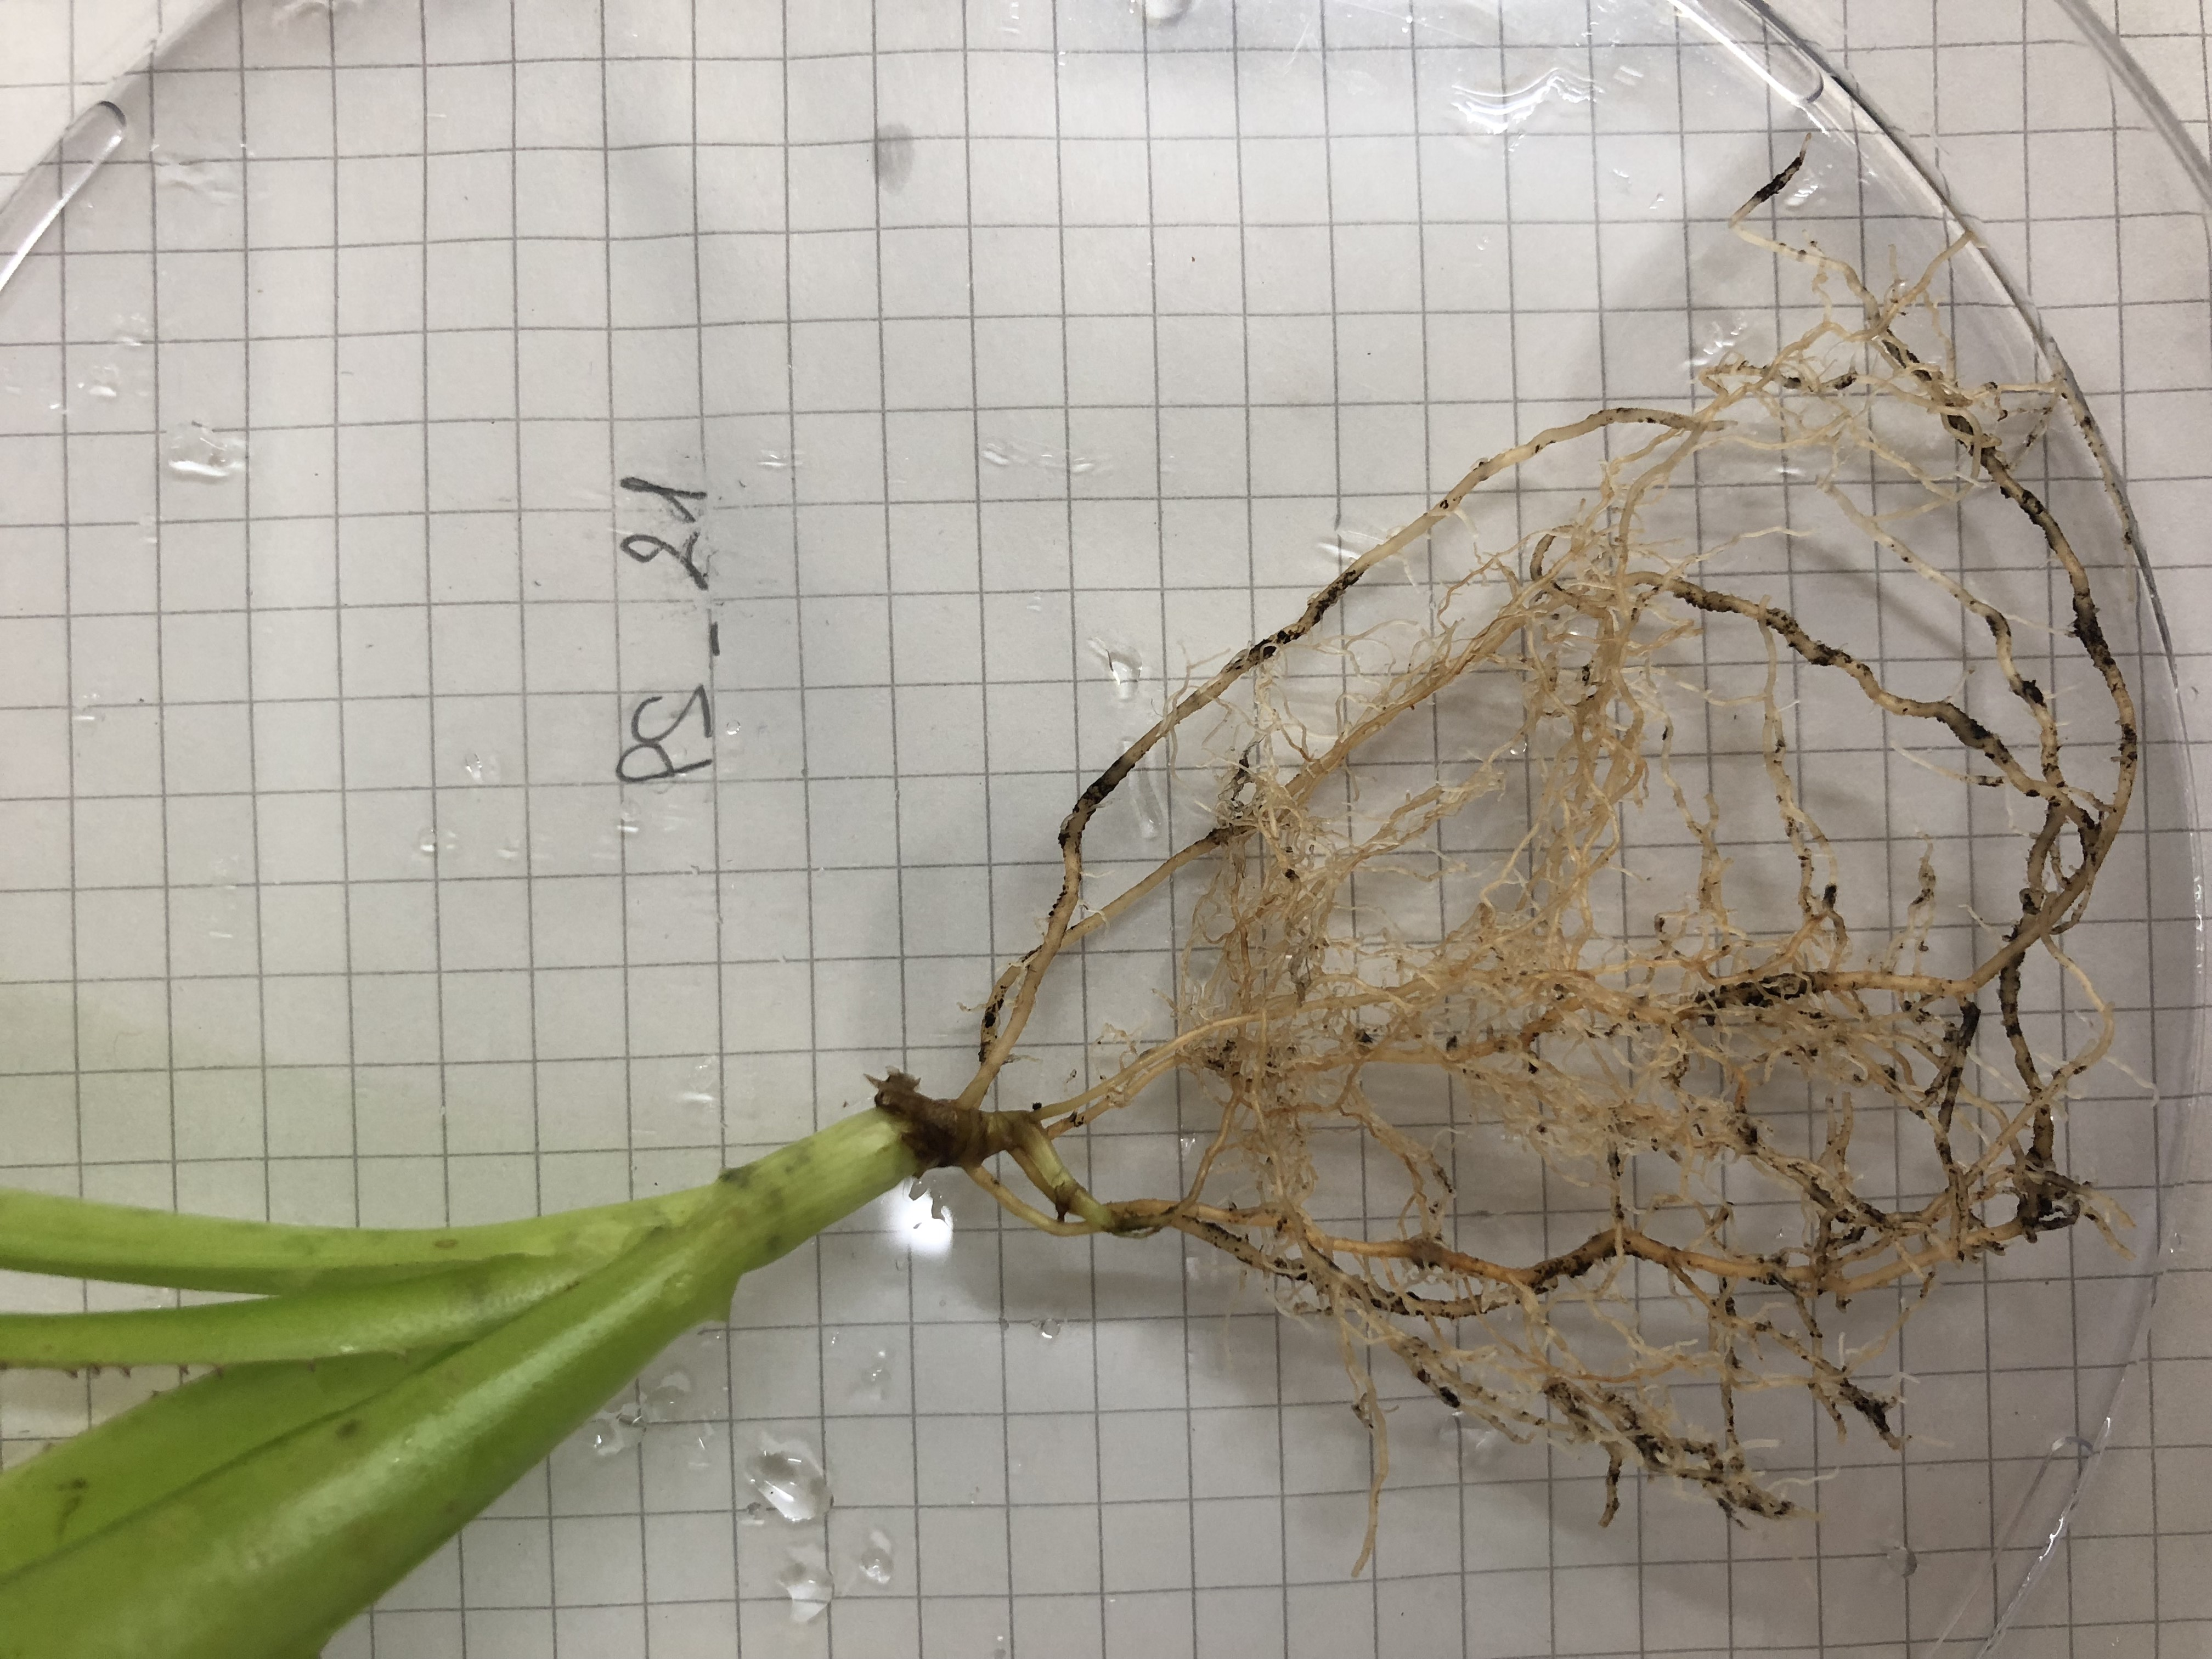
\includegraphics[width=0.5\linewidth]{document/trait/rootmorpho/bromeroot} 

}

\caption{Complex bromeliad adventitious root system}\label{fig:bromeroot}
\end{figure}

\normalsize

\textbf{BEWARE:} The \texttt{Transparent} scan window is smaller than the normal mode scan. The actual scanned zone is showed \ref{fig:scantransp} and you must make sure that you roots are well placed within this area.

\scriptsize

\begin{figure}

{\centering 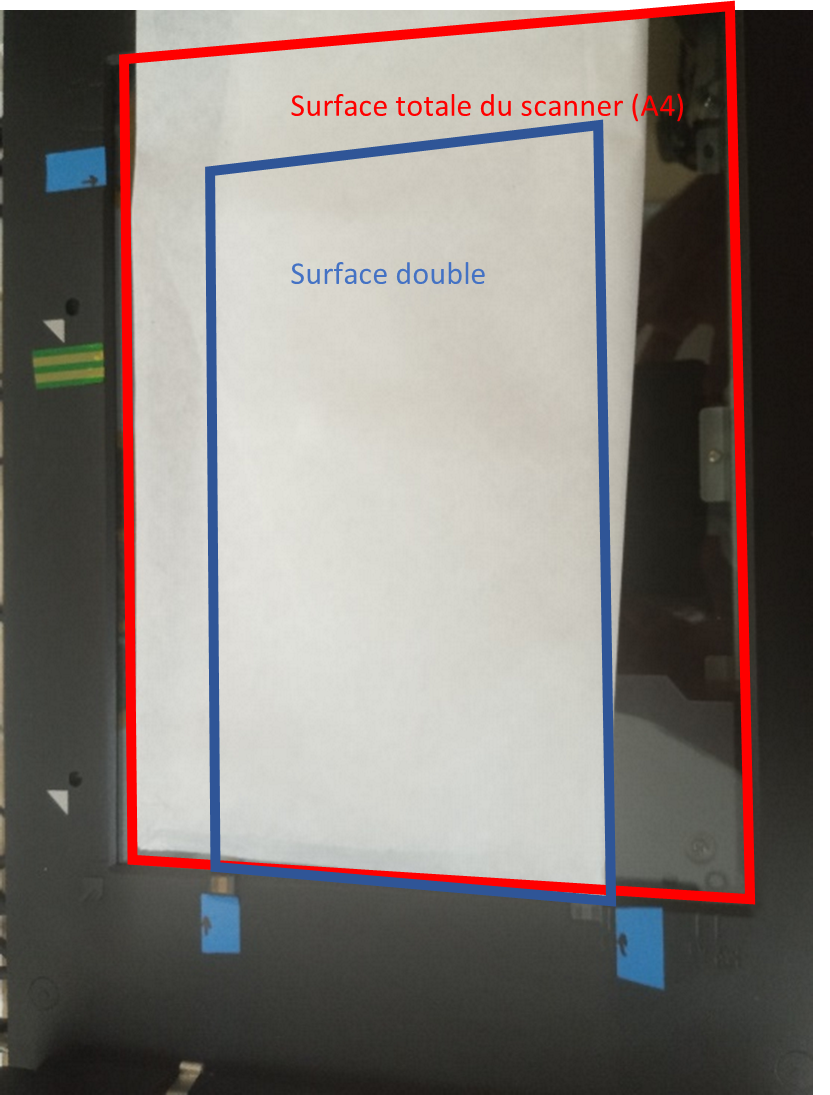
\includegraphics[width=0.5\linewidth]{document/trait/rootmorpho/scan_transp} 

}

\caption{Flat (red) and Transparent (blue) scan zone of EPSON's V800 scanner}\label{fig:scantransp}
\end{figure}

\normalsize

\hypertarget{image-processing}{%
\subsection{Image processing}\label{image-processing}}

To analyze with winrhizo, you can either make it manually, one image at a time and by drawing rectangles around the roots you want to analyze.
However, when having a lot of scans you might want to automatize the process using the \texttt{batch} option.
If this is your choice, make sure that your images only contain roots!! Sometimes you will have to remove some parts of the scans to leave only roots in your images.
For instance, this \ref{fig:bromescan} is the scan from bromeliads roots. We can see the water-filled petri dishes border on the scan and this will be an issue for automatized Winrhizo analysis.

\scriptsize

\begin{figure}

{\centering 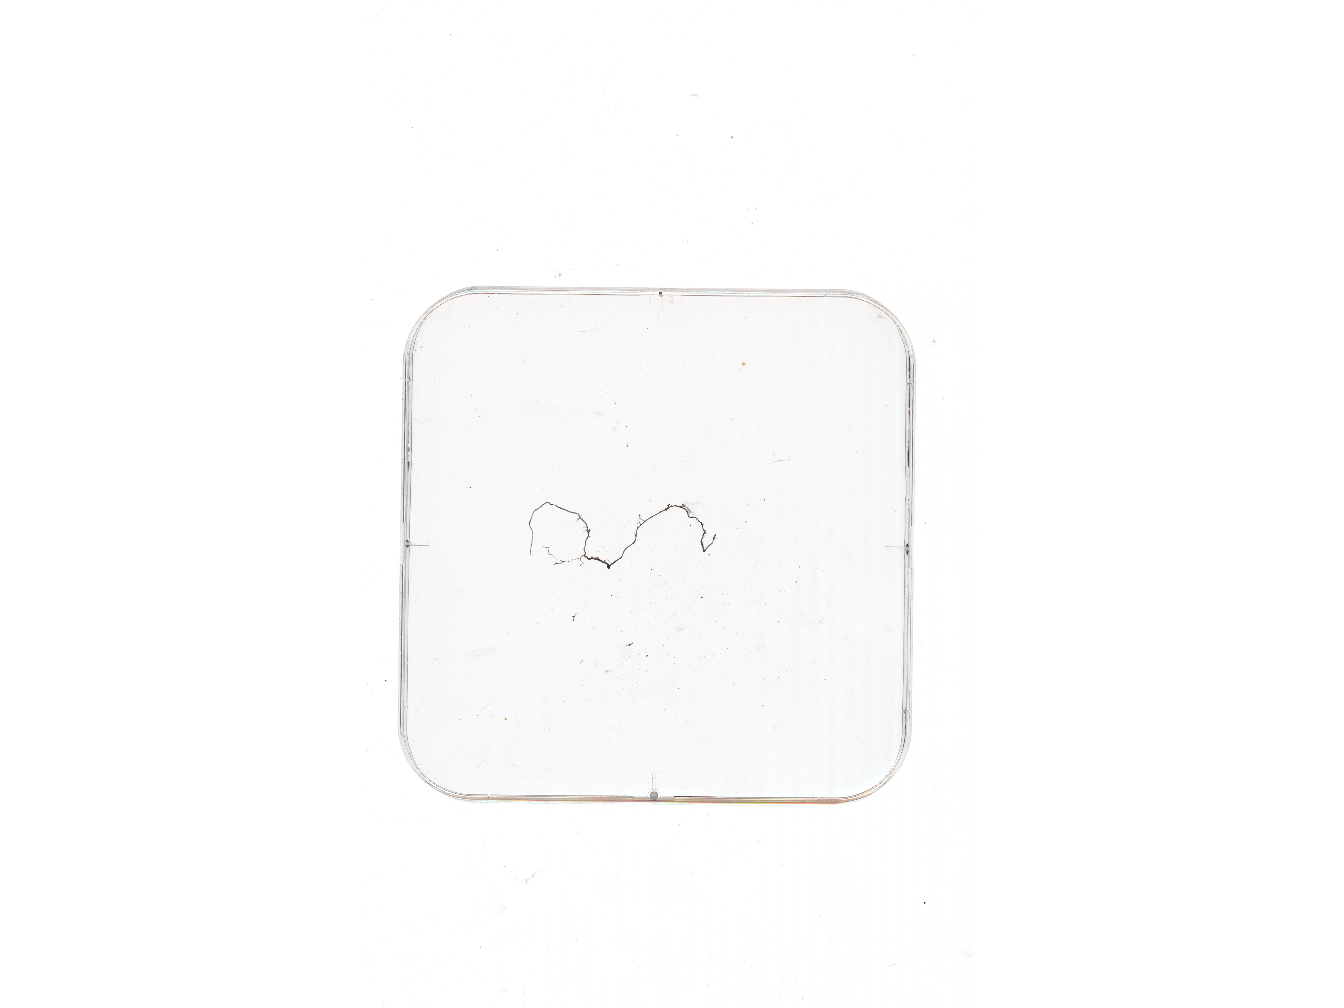
\includegraphics[width=0.5\linewidth]{MyBook_files/figure-latex/bromescan-1} 

}

\caption{Scan of a bromeliad root system in water-filled petri dish}\label{fig:bromescan}
\end{figure}

\normalsize

To re-crop these images we use the freeware \texttt{XnConvert}.
The petri dish has always been placed in the same place using a stencil \ref{fig:scanstencil} on the scan window, enabling us to recrop all scans to the same size.
Detailed \texttt{XnConvert} tutorial is available \href{document/software/XnConvert/XnConvert_tuto.pdf}{HERE}.

\scriptsize

\begin{figure}

{\centering 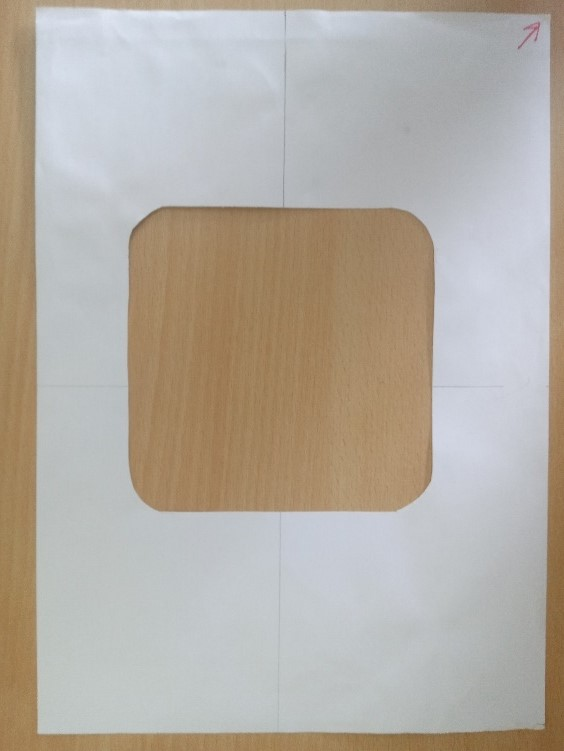
\includegraphics[width=0.5\linewidth]{document/trait/rootmorpho/squre_stencil} 

}

\caption{Stencil used for inwater root scans}\label{fig:scanstencil-1}
\end{figure}
\begin{figure}

{\centering 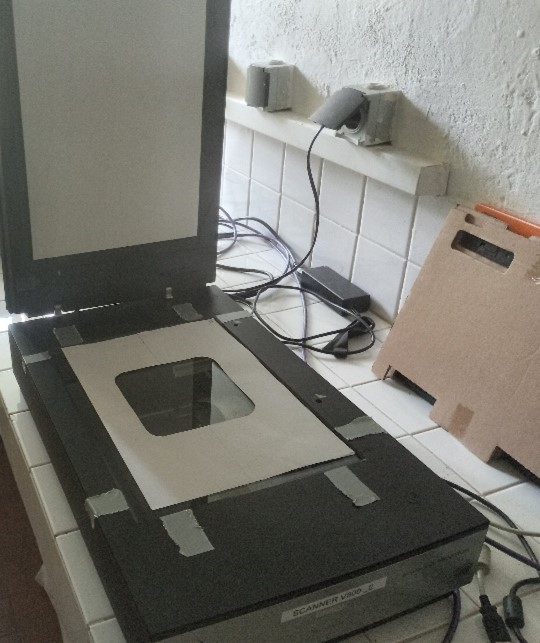
\includegraphics[width=0.5\linewidth]{document/trait/rootmorpho/squre_stencil2} 

}

\caption{Stencil used for inwater root scans}\label{fig:scanstencil-2}
\end{figure}

\normalsize

\hypertarget{winrhizo}{%
\subsection{WinRhizo}\label{winrhizo}}

\hypertarget{installation}{%
\subsubsection{Installation}\label{installation}}

The winrhizo software is contained on a CD (ask \href{https://docs.google.com/spreadsheets/d/1EqjCVr6w7fykUJtLOVwSNBucNfFGbiYXGlRcoL-s7V8/edit\#gid=0}{\textbf{Eliane Louisanna}}.
To be used you need to copy the software from the disk to your computer and install the protection key drivers (also on the CD). Once installed you don't need the CD to run the software but the protection key must be plugged.
Unplugging it will prevent any use of the software.

\hypertarget{startup}{%
\subsubsection{Startup}\label{startup}}

\hypertarget{first-analysis}{%
\subsubsection{First analysis}\label{first-analysis}}

Once you have acquired your images and launched winrhizo you can start to analyze your scans.
To display a single scan, click \emph{Image} -\textgreater{} \emph{Origin} -\textgreater{} \emph{From File}.
Then you can click the \emph{acquisition }icon \textbf{PIC}.
This will open a standard document opening window.
Then you browse normally to find the wanted scan.
Make sure that you are looking for the goor format, by default, winrhizo display \texttt{.TIFF}.
When you open it, winrhizo display the targeted image and you can then click on it (analyze whole image) or make a selection (only selected region) to start an analysis.

When an image or region is analyzed, winrhizo display the \emph{sample identification} window which allows you to enter information about the sample.
These information will be saved with the measurements data.
In this window click \emph{OK} to do the analysis or \emph{Cancel} to abort it.

After you clicked \emph{OK}, winrhizo starts the analysis (can be stopped pressing \emph{S}).
When done, winrhizo is ready to save the data but a file must be opened or created first.
Winrhizo display a window which asks wether to \emph{open one}, \emph{create one} or \emph{save nothing}.
Selecting \emph{create one} will create a new \texttt{.TXT} file to store analysis data (more info about output \protect\hyperlink{output}{here}).
Selecting \emph{open one} will allow you to open a pre-existing file to add the new measurements at the end of this file.
Clicking on \emph{save nothing}, guess?

In the image, you can now see which roots have been analyzed.
This have a skeleton line over them.
The absence of this skeleton indicates that these roots have not been analyzed.
This can be due to non-optimal pixel classification (see more about it \protect\hyperlink{pixel-classification}{here}).

WELL DONE! You just analyze your first picture!

You can practice with scans available \protect\hyperlink{resources}{here}

\hypertarget{calibration}{%
\subsubsection{Calibration}\label{calibration}}

If not calibrated (associated with a scale), winrhizo will display results in pixels.
\texttt{.TIFF} files have an embedded scale, automatically detected by winrhizo.
Check on your results if they are in px (pixels), in (inches) or cm (centimeters).

However, you can sometimes have uncalibrated files (mistakes or images from camera).
Thus, you will need to ``manually'' calibrate your image.
Winrhizo calibration files are saved as \texttt{.CAL}. In the \emph{Calibration} menu you can load pre-existing calibration files.
You will find the \texttt{calib\_imge.TIFF} \href{document/trait/rootmorpho/calib_imge.TIF}{here}.
To make your calibration at any DPI, you can print this image and scan it at the wanted DPI.
The black square in the image delimit a white 1x1cm square.
Loading this image in winrhizo, you can click on \emph{calibration} -\textgreater{} \emph{pixel size method} -\textgreater{} \emph{object of known dimension} -\textgreater{} \emph{1 image} -\textgreater{} width=1 , height=1, border=0.35, units=cm -\textgreater{} \emph{Ok}

Then, winrhizo will propose you to save the calibration in a \texttt{.CAL} file that can be loaded later and used for all your images at a given resolution. \textcolor{red}{DO NOT NAME YOUR FILE Scanner.cal}.
Please, when you create a \texttt{.CAL} at a previously not used resolution, store a copy of the calibration file \href{document/software/Winrhizo/}{here} so that your work helps your successors!!

\hypertarget{batch}{%
\subsubsection{Batch}\label{batch}}

We saw how to analyze a \protect\hyperlink{first-analysis}{single picture or region} but you might have numerous scans to analyze and want to automatize this process.
To do so you will give winrhizo a \emph{batch} (i.e.~a folder) containing any number of images you want.

\hypertarget{pixel-classification}{%
\subsubsection{Pixel classification}\label{pixel-classification}}

Pixel classification is how winrhizo discriminate between actual ``root'' pixels and scan background.
To do this distinction you have several options presented in \emph{Analysis} -\textgreater{} \emph{Root \& Background Distinction} menu.
This distinction is made grey levels and can either be set to \emph{automatic} or \emph{manual}.
Automatic option either sets a global threshold (default) of grey value at which the pixel is attributed to roots or background or it can be used with \emph{lagarde} options which consider local region (region size can be defined in pixels) of the picture and associate different threshold values.
We don't recommend the use of \emph{lagarde} option but a careful cleaning of your roots and high quality scans.
However you can test different options with some of your scans to chose the best options.
It is also important to tell the software if your scans are Dark roots on White background or the contrary.

\hypertarget{output}{%
\subsubsection{Output}\label{output}}

\hypertarget{resources}{%
\section{Resources}\label{resources}}

\hypertarget{hydraulics}{%
\chapter{Hydraulics}\label{hydraulics}}

\hypertarget{leaf-turgor-loss-point-pi_tlp}{%
\section{\texorpdfstring{Leaf turgor loss point, \(\pi_{tlp}\)}{Leaf turgor loss point, \textbackslash pi\_\{tlp\}}}\label{leaf-turgor-loss-point-pi_tlp}}

We assessed the leaf turgor loss point, \(\pi_{tlp}\) in MPa, from a previously established relationship with the osmotic potential at full hydration, \(\pi_{osm}\) in MPa. \(\pi_{osm}\) is linked to the equilibrium solute concentration value \(C_0\) (in mmol.kg\^{}\{-1\}) directly measured with a vapor pressure osmometer (Vapro 5600, Wescor, Logan, UT). This is referred as the \emph{osmometer method} (Bartlett et al.~2012a; Maréchaux et al.~2016).

\hypertarget{materials}{%
\subsection{Materials}\label{materials}}

\begin{itemize}
\tightlist
\item
  Vapor pressure osmometer (Vapro 5520, Wescor, Logan, UT)
\item
  Vapro software (Vapro Lab Report)
\item
  Fridge
\item
  Liquid Nitrogen
\item
  Ziplock bag\\
\item
  Paper towel
\item
  Distilled water
\item
  Metal tea ball
\item
  Tin foil
\item
  Needle\\
\item
  Liquid nitrogen gloves + goggles
\item
  Liquid nitrogen contenant
\item
  2 Tweezers
\item
  Cork borer
\end{itemize}

\hypertarget{methods}{%
\subsection{Methods}\label{methods}}

\hypertarget{installing-vapro-for-measurements}{%
\subsubsection{Installing Vapro for measurements}\label{installing-vapro-for-measurements}}

\begin{itemize}
\tightlist
\item
  Turn on Vapro the day before for the thermocouple's stability
\item
  Test Water Quality \emph{cf Vapro\_cheatsheet}
\item
  Clean
\item
  Calibration \emph{cf Vapro\_cheatsheet}
\item
  Control tests \emph{cf Vapro\_cheatsheet}
\item
  Verify temperature
\item
  Always have the black diamond at the center of the display
\end{itemize}

Used daily:
* clean beforehand
* select automatic mode (10 runs)

\hypertarget{sampling-on-the-field}{%
\subsubsection{Sampling on the field}\label{sampling-on-the-field}}

\begin{itemize}
\tightlist
\item
  Collect at least 3 healthy mature leaves on branch
\item
  Place them in sample ziplock bag with:

  \begin{itemize}
  \tightlist
  \item
    wet paper towel
  \item
    Exhale in bag to saturate in CO\textsubscript{2}
  \item
    Annotate bag with sample information
  \end{itemize}
\item
  Zip bag and stock in cooler
\end{itemize}

\hypertarget{lab-measurements}{%
\subsubsection{Lab measurements}\label{lab-measurements}}

\hypertarget{field-day}{%
\paragraph{Field day}\label{field-day}}

\begin{itemize}
\tightlist
\item
  Recut branch under water
\item
  Replace in ziplock bag with wet paper towel
\item
  Put 24h in fridge to hydrate overnight
\end{itemize}

\hypertarget{n1-field-day}{%
\paragraph{N+1 Field day}\label{n1-field-day}}

Vapro:

\begin{itemize}
\tightlist
\item
  check distilled water in vapro reservoir
\item
  clean
\item
  select automatic mode (10 runs)
\item
  make sure vapro software is on
\end{itemize}

Sample measurement:

\begin{itemize}
\tightlist
\item
  Sample from a leaf a 5 mm disc with a cork borer: \emph{avoid 1\textsuperscript{st} and 2\textsuperscript{nd} order veins to avoid apoplastic dilution that would lead to less negative osmometer values}
\item
  Wrap disc in tin foil
\item
  Immerse in liquid nitrogen for at least 2 min using metal tea ball
\item
  Puncture 10-15 times with needle
\item
  Place in vapro chamber
\end{itemize}

In total, disc are exposed to air for less than 40 seconds for all the steps.

\begin{itemize}
\item
  Record value C\textsubscript{0} when the difference between consecutive 2-min measurements fell below strictly 5 mmol.kg\textsuperscript{-1} after at least three runs.
\item
  If error! or Nr\_Run \textgreater{} 10 :
\item
  try a 2\textsuperscript{nd} cycle with same leaf
\item
  try a 3\textsuperscript{rd} cycle with another leaf
\item
  otherwise record \emph{NA}
\item
  Beware of the stuck leaf inside the vapro! If so \emph{cf Vapro\_cheatsheet}
\end{itemize}

\hypertarget{end-measurements}{%
\paragraph{End measurements}\label{end-measurements}}

Clean Vapro

For more information on the vapro machine, please refer to the \emph{vapro cheatsheet} in the machine category.

\hypertarget{leaf-midday-water-potential}{%
\section{Leaf midday water potential}\label{leaf-midday-water-potential}}

\hypertarget{pressure-chamber-method}{%
\subsection{Pressure chamber method}\label{pressure-chamber-method}}

\hypertarget{psychrometry-method}{%
\subsection{Psychrometry method}\label{psychrometry-method}}

\hypertarget{relative-water-content-rwc}{%
\section{Relative water content RWC (\%)}\label{relative-water-content-rwc}}

\hypertarget{material}{%
\subsection{Material}\label{material}}

\emph{Ziplock bag
}Paper towel
\emph{Distilled water
}Fridge
\emph{Analytical balance
}Sharpie
\emph{cooler
}envelop

\hypertarget{method}{%
\subsection{Method}\label{method}}

Before going on the field:
* write individual code on ziplock bag
* preweight ziplock bag

On the field:
* collect leaf
* clean leaf with clean paper towel
* place leaf in preweighted corresponding ziplock bag
* place bag in cooler for transport to the lab

In the lab:
* weight the closed ziplock with the leaf (\emph{fresh weight})
* delicately take the leaf out of the bag, wrap it in moist paper towel and place the wrap back in the ziplock bag
* place ziplock bag in the fridge during 24 hours
* 24 hours later, take out the leaf and wipe off water excess
* weight re-hydrated leaf (\emph{saturated weight})
* place leaf in envelop for oven-drying during at least 72h
* weight dry leaf (\emph{dry weight})

Calculate RWC (\%):

RWC = \(\frac{(fresh\ weight-dry\ weight)}{(saturated\ weight-dry\ weight)}\) X 100

From Sapes et al 2020 and Barrs \& Weatherley 1962.

\hypertarget{gmin}{%
\section{gmin}\label{gmin}}

\hypertarget{gs}{%
\section{gs}\label{gs}}

\hypertarget{fluorescence}{%
\chapter{Fluorescence}\label{fluorescence}}

Fluorescence measurements are made with the \href{document/machine/MiniPAM\%20II/minipamexp.pdf}{\texttt{MiniPAM\ II}} fluorometer.
It is used to assess the efficiency of plant photosystems to convert light into chemical energy.

\href{document/trait/fluorescence/Maxwell\%20and\%20Johnson\%20-\%202000\%20-\%20Chlorophyll\%20fluorescence—a\%20practical\%20guide.pdf}{Maxwell and Johnson \emph{2000}} provided a good synthesis of the theories behind these measurements.

A french and detailed version of Fluorescence measurements is available \href{document/machine/MiniPAM\%20II/Manuel\%20Mini-PAM\%20II6300_\%20Maxime\%20B}{here}

\hypertarget{theory}{%
\section{Theory}\label{theory}}

We will try to summarize it a bit here.
Light energy is either converted into \texttt{Photochemical\ energy}, \texttt{fluorescence} or \texttt{heat}.
Measuring fluorescence can give information about the other if we control one (i.e.~photochemistry).

We use the \texttt{Kautsky\ effect}, a variation of the \texttt{fluorescence} pattern when exposing the leaf to light.
When passing from darkness to light, photon will saturate the plant photosystem II and e\^{}- acceptors.
The PSII are sayed ``closed'' until e\textsuperscript{-} go down the reaction chain.

Thus, for a few seconds, the system cannot do photochemistry and only emits fluo (measurable) and heat!!!

After this period, the fluorescence starts to fall again ==\textgreater{} \texttt{fluorescence\ quenching}

Because :

1 - e- transfer away from the PSII increases with light activated enzymes : \textbf{photochemical quenching}

2 - Heat energy estimation : \textbf{Non-photochemical quenching}

\textasciitilde{} 15 to 20 min are needed to reach the equilibrium but it varies between species.

For usefull informations, we need to supress one of the 2 (typically 1).
Indeed, if no photochemical quenching (PQ), then we only have non-photochemical quenching (NPQ).

We thus use the \texttt{light\ doubling\ technique}.

An high intensity-short duration flash closes all PSII.

During this flash, the fluorescence yield reach values attained with no NPQ (\(F_m\)).

\(F_0\) is the fluorescence level when no actinic light (darkening + far red to open reaction centers).

\(F_t\) is the steady state of fluorescence in actinic light.

NPQ can too change with time and this is reflected as \(F_m\) changes when PQ is off/negligible.

We can then calculate :

\(\phi _{SII} = \frac{F'_m-F_t}{F'_m}\) which is the proportion of light absorbed by PSII chlorophyll and used for photochemistry.

and :

\(qP = \frac{F'_m-F_t}{F'_m-F'_0}\) the proportion of closed PSII reaction center, it increases with plant stress.

\(F_v/F_m=\frac{\phi _{PSII}}{qP}=\frac{F'_m-F'_0}{F'_m}\) or with \(F°_m\) and \(F°_0\) in the dark adapted state.

\hypertarget{fv.fm}{%
\section{Fv.Fm}\label{fv.fm}}

To measure Fv/Fm with the MiniPAM you have to use the dark leaf clip and place one on the target leaf for 30 minutes dark adaptation.
Then press record on the MiniPAM screen to create a new data entry.
And, finally just insert the optical fiber in the leaf clip, open it and press Fv/Fm on the MiniPAM screen.
You can either note the displayed value manually or extract it later with the MiniPAM associated software \href{https://www.walz.com/products/chl_p700/mini-pam-II/downloads.html}{\texttt{Wincontrol}}.
If you chose the later, do note the correspondence between your subject ID and the record created by the MiniPAM.

\hypertarget{etrmax}{%
\section{ETRmax}\label{etrmax}}

To measure ETRmax, a leaf is quasi-dark acclimated for 150s in an opaque plastic bag before gradual exposition to increasing PAR values in twelve 30s steps ranging from 50 to 3000 µmol photon m-2 s -1.
ETR is obtained using the WinControl-3 software (Walz, Effeltrich, Germany) and an R script chosing between two models (Reg1, with photoinhibition, and Reg2, without) given by Platt et al.~(1980).

\begin{itemize}
\tightlist
\item
  Attach the fibre optic cable to the leaf clip holder and use a stand if necessary.
\item
  Hold the leaf clip holder firmly to the sheet to be measured (avoid the ribs if possible).
\item
  Place the leaf clip holder in the dark for 150 seconds: cover it so that it is not in contact with the ambient light (quasi-dark adaptation)
\item
  On the screen (Basic data), press the arrow pointing downwards until you see the Light curve, and then press \textbf{START}.
\item
  At the end of the measurement, the curve and all data will be saved automatically.
\item
  The only way to retrieve the data is to note the time the RLC was started.
\end{itemize}

For the curves, the plant must remain in the dark until the end of the curve and above all not move the leaf clip holder so that the flash of light remains in the same place.

\hypertarget{getting-data-out-of-the-minipam-ii}{%
\section{Getting data out of the MiniPAM II}\label{getting-data-out-of-the-minipam-ii}}

WinControl-3 is a mandatory software to deal with miniPAM II data and can be downloaded \href{https://www.walz.com/products/chl_p700/mini-pam-II/downloads.html}{here}.
Plug the MiniPAM II to your computer and launch WinControl.
When you have a good version of WinControl, a window opens with the MINIPAM data.
To view the data, press \textbf{MEMORY} and a list of data is displayed.
To download the data shown on the list :

\textbf{MEMORY}→ Select by pressing what you want to download → Download selected files → Check ``clear existing data in WinControl before download→ Ok.
(Especially for the light curve data. If you check''merge with current data'' all data will be merged and then you lose the ETRmax1 and ETRmax2 values)

To view the downloaded data, press \textbf{Report}.
\textbf{Report} is only an intermediate step to view the data.
Let some time before downloading reported data for RLC so that the software can compute Reg1 and 2 models.
To download data from several pages you need to check ``merge withcurrent data in WinControl''.
(Not recommended for CDNs for fear of losing some data)

To save in \texttt{.csv}, Report → Select all → right clic → Export all→ Ok → file name → save

\hypertarget{process-with-r-scripts}{%
\section{Process with R scripts}\label{process-with-r-scripts}}

This is done using the \texttt{merge\_minipam} and \texttt{minipam} functions of the \texttt{EcophyCofog} package written by Tristan LAFONT RAPNOUIL and hosted on \href{https://github.com/LafontRapnouilTristan/EcophyCofog}{github}.

See \protect\hyperlink{ecophycofog-package}{EcophyCofog Package} for more information on the package.

First, if your download resulted in several \texttt{.csv} files, you have to run the \texttt{merge\_minipam}.
Place all your files (and only them!!) in a folder.

\scriptsize

\begin{Shaded}
\begin{Highlighting}[]
\FunctionTok{library}\NormalTok{(EcophyCofog)}
\NormalTok{input\_path }\OtherTok{\textless{}{-}}\NormalTok{ PATH\_TO\_THE\_FOLDER}
\NormalTok{filename }\OtherTok{\textless{}{-}}\NormalTok{ NAME\_OF\_THE\_MERGED\_OUTPUT}
\FunctionTok{merge\_minipam}\NormalTok{(input\_path, filename)}
\end{Highlighting}
\end{Shaded}

\normalsize

Then you'll run the \texttt{minipam} function on your merged file.
NOTE that you can also chose not to merge your files and process them individually with \texttt{minipam}.

To run this function you'll need a \emph{ID\_match} \texttt{.csv} file.
It's a file with 4 columns: \textbf{ID} (ID of measured plant, leaf, sample), \textbf{Date} (date of the measurement, DD:MM:YYYY format), \textbf{Time} (Hour at which started the measurement HH:MM format), \textbf{REC} (the MiniPAM record ID)

\scriptsize

\begin{Shaded}
\begin{Highlighting}[]
\FunctionTok{library}\NormalTok{(EcophyCofog)}
\NormalTok{Name\_of\_the\_input\_file }\OtherTok{\textless{}{-}}\NormalTok{ NAME\_OF\_YOUR\_MERGED\_FILE}
\NormalTok{input\_path }\OtherTok{\textless{}{-}}\NormalTok{ PATH\_TO\_SAID\_FILE}
\NormalTok{path\_to\_ID\_match }\OtherTok{\textless{}{-}}\NormalTok{ PATH\_TO\_YOUR\_ID\_MATCH\_FILE}
\FunctionTok{minipam}\NormalTok{(Name\_of\_the\_input\_file, input\_path, path\_to\_ID\_match)}
\end{Highlighting}
\end{Shaded}

\normalsize

Running this will produce a table with FvFm and ETRmax values for all your samples.
It'll additionally produce graphics of the RLC (ETR\textasciitilde PAR).

\hypertarget{gaz-fluxes-and-exchanges}{%
\chapter{Gaz fluxes and exchanges}\label{gaz-fluxes-and-exchanges}}

Gas exchanges can be measured using the CIRAS-3 Analyser (PP Systems, Amesbury, U.S.A).

Using a leaf clip with an enclosed chamber allows to measure CO2 and H2O fluxes in the chamber.

\hypertarget{ecophycofog-package}{%
\chapter{EcophyCofog Package}\label{ecophycofog-package}}

A package to handle routinely produced raw outputs of the CIRAS-3, MINIPAM II and PSYPRO of EcoFog's ecophysiology lab.

Package written by Tristan LAFONT RAPNOUIL and hosted on \href{https://github.com/LafontRapnouilTristan/EcophyCofog}{github}.
Can be installed running:

\begin{verbatim}
install.packages("devtools")
library(devtools)
install_github("https://github.com/LafontRapnouilTristan/EcophyCofog")
\end{verbatim}

\hypertarget{utilitaries}{%
\section{Utilitaries}\label{utilitaries}}

\hypertarget{library}{%
\subsection{Library}\label{library}}

Used to load install (if required) and load multiple package at once.

usage:

\scriptsize

\begin{Shaded}
\begin{Highlighting}[]
\NormalTok{EcophyCofog}\SpecialCharTok{::}\FunctionTok{Library}\NormalTok{(}\FunctionTok{c}\NormalTok{(}\StringTok{"pckg1"}\NormalTok{, }\StringTok{"pckg2"}\NormalTok{, }\StringTok{"pckg3"}\NormalTok{))}
\end{Highlighting}
\end{Shaded}

\normalsize

\hypertarget{notin}{%
\subsection{NotIn}\label{notin}}

A custom operator to test the differences between vectors.

\scriptsize

\begin{Shaded}
\begin{Highlighting}[]
\NormalTok{x }\OtherTok{\textless{}{-}} \FunctionTok{c}\NormalTok{(}\StringTok{"a"}\NormalTok{, }\StringTok{"b"}\NormalTok{, }\StringTok{"c"}\NormalTok{)}
\NormalTok{y }\OtherTok{\textless{}{-}} \FunctionTok{c}\NormalTok{(}\StringTok{"d"}\NormalTok{, }\StringTok{"a"}\NormalTok{, }\StringTok{"e"}\NormalTok{)}
\NormalTok{x }\SpecialCharTok{\%notin\%}\NormalTok{ y}
\end{Highlighting}
\end{Shaded}

\normalsize

\texttt{{[}1{]}\ FALSE\ \ TRUE\ \ TRUE}

\hypertarget{xtract_legend}{%
\subsection{xtract\_legend}\label{xtract_legend}}

Store the legend of a ggplot object.

\scriptsize

\begin{Shaded}
\begin{Highlighting}[]
\NormalTok{legend }\OtherTok{\textless{}{-}} \FunctionTok{xtract\_legend}\NormalTok{(myggplot)}
\end{Highlighting}
\end{Shaded}

\normalsize

\hypertarget{dummy_data}{%
\subsection{dummy\_data}\label{dummy_data}}

Create a meaningless numeric data frame for testing things.

\scriptsize

\begin{Shaded}
\begin{Highlighting}[]
\NormalTok{data }\OtherTok{\textless{}{-}} \FunctionTok{dummy\_data}\NormalTok{(}\AttributeTok{nbcol =} \DecValTok{4}\NormalTok{, }\AttributeTok{nbrow =} \DecValTok{100}\NormalTok{)}
\end{Highlighting}
\end{Shaded}

\normalsize

\hypertarget{minipam}{%
\section{MiniPAM}\label{minipam}}

\hypertarget{merge_minipam}{%
\subsection{merge\_minipam}\label{merge_minipam}}

Merge several miniPAM output files.
All files should be stored in one folder, and only them!!
See \protect\hyperlink{fluorescence}{Fluorescence} for more details.

\scriptsize

\begin{Shaded}
\begin{Highlighting}[]
\FunctionTok{library}\NormalTok{(EcophyCofog)}
\NormalTok{input\_path }\OtherTok{\textless{}{-}}\NormalTok{ PATH\_TO\_THE\_FOLDER}
\NormalTok{filename }\OtherTok{\textless{}{-}}\NormalTok{ NAME\_OF\_THE\_MERGED\_OUTPUT}
\FunctionTok{merge\_minipam}\NormalTok{(input\_path, filename)}
\end{Highlighting}
\end{Shaded}

\normalsize

\hypertarget{minipam-1}{%
\subsection{minipam}\label{minipam-1}}

Take as input a csv dataframe containing output of the minipam.
For ETR and Fv/Fm measurements only.
And return clean files containing each type of measurements + the ETR curves.

\scriptsize

\begin{Shaded}
\begin{Highlighting}[]
\FunctionTok{library}\NormalTok{(EcophyCofog)}
\NormalTok{Name\_of\_the\_input\_file }\OtherTok{\textless{}{-}}\NormalTok{ NAME\_OF\_YOUR\_MERGED\_FILE}
\NormalTok{input\_path }\OtherTok{\textless{}{-}}\NormalTok{ PATH\_TO\_SAID\_FILE}
\NormalTok{path\_to\_ID\_match }\OtherTok{\textless{}{-}}\NormalTok{ PATH\_TO\_YOUR\_ID\_MATCH\_FILE}
\FunctionTok{minipam}\NormalTok{(Name\_of\_the\_input\_file, input\_path, path\_to\_ID\_match)}
\end{Highlighting}
\end{Shaded}

\normalsize

\hypertarget{ciras-3}{%
\section{CIRAS-3}\label{ciras-3}}

\hypertarget{merge_ciras}{%
\subsection{merge\_ciras}\label{merge_ciras}}

Used to merge all ciras output of a foled into one file.

\emph{path\_to\_xls} a character string with your path to all your ciras \texttt{.xls} output.
Their name must always end as \_treatment\_sampleID.xls (e.g.~CIRAS\_3\_Aechmea m \_DP\_1.xls).
\emph{skip}: the number of useless rows at the top of your \texttt{.xls} file, Jean-Yves Goret template have three.

\scriptsize

\begin{Shaded}
\begin{Highlighting}[]
\FunctionTok{merge\_ciras}\NormalTok{(path\_to\_xls, }\AttributeTok{skip =} \DecValTok{3}\NormalTok{)}
\end{Highlighting}
\end{Shaded}

\normalsize

\hypertarget{psypro}{%
\section{PSYPRO}\label{psypro}}

\hypertarget{psypro-1}{%
\subsection{psypro}\label{psypro-1}}

Transform psypro output files into csv dataframe with mean water potential of your triplicate.
\texttt{param} \emph{usedset} the predetermined name of your set 0,1,2 or 3.
\texttt{param} \emph{lim} min and max values expected out of the psypro for you samples.
Used to standardized graphs for faster reading.
Discuss with lab members to understand!!
\texttt{param} \emph{ID\_vec} a vector of length 8 (number of sensors) with your samples' ID.
Empty sensors are named 0!!
\texttt{param} \emph{path\_to\_calibration} path to you calibration file.
\texttt{param} \emph{psypro\_output} path to your psypro output.

\scriptsize

\begin{Shaded}
\begin{Highlighting}[]
\FunctionTok{psypro}\NormalTok{(usedset, }\AttributeTok{lim =} \FunctionTok{c}\NormalTok{(}\SpecialCharTok{{-}}\DecValTok{3}\NormalTok{, }\DecValTok{2}\NormalTok{), ID\_vec, path\_to\_calibration,}
\NormalTok{    psypro\_output)}
\end{Highlighting}
\end{Shaded}

\normalsize

\hypertarget{pasco}{%
\section{PASCO}\label{pasco}}

\hypertarget{pasco_transfo}{%
\subsection{PASCO\_transfo}\label{pasco_transfo}}

An earlier version of PASCO\_transfo2, should not be used anymore.

\hypertarget{pasco_transfo2}{%
\subsection{PASCO\_transfo2}\label{pasco_transfo2}}

Process the PASCO probe output csv to get the gasfluxes.

\texttt{param} \emph{data} a data frame output from Sparkview (usually read from .csv)
\texttt{param} \emph{ech} a character vector with either the probe or sample name
\texttt{param} \emph{name\_run} a character vector with the name of all your runs (e.g., c(``stab1'',``RECO'',``NEE''))
\texttt{param} \emph{select} a numeric vector of the runs you want to keep (e.g., c(2,3))
\texttt{param} \emph{A} the Area
\texttt{param} \emph{V} the Volume

\scriptsize

\begin{Shaded}
\begin{Highlighting}[]
\FunctionTok{PASCO\_transfo2}\NormalTok{(data, ech, name\_run, select, }\AttributeTok{A =} \DecValTok{1}\NormalTok{, }\AttributeTok{V =} \DecValTok{5}\NormalTok{)}
\end{Highlighting}
\end{Shaded}

\normalsize

\hypertarget{pcr-layout}{%
\section{PCR layout}\label{pcr-layout}}

Functions to create excel files containing the PCR plate layout (with controls and all) from your sample list.
Both for sample names and then tags combination.

\hypertarget{plate_layout}{%
\subsection{plate\_layout}\label{plate_layout}}

\texttt{param} \emph{samples} a vector containing all your samples ID, they will fill the plate in the order they are in this vector, when having replicates for one sample, plz index them as ``SampleName 1'' to ``SampleName N'' and not ``SampleName\_X'' or ``SampleName.X''.
\texttt{param} \emph{proj} name of your project to name your plates as : ``proj-PLx''
\texttt{param} \emph{name\_file} a name to your output file
\texttt{param} \emph{save\_file\_path} path to where you want to save the excel output
\texttt{param} \emph{starting\_plate\_number} where from start plate numbering

\scriptsize

\begin{Shaded}
\begin{Highlighting}[]
\FunctionTok{plate\_layout}\NormalTok{(samples, proj, name\_file, save\_file\_path, }\AttributeTok{starting\_plate\_number =} \DecValTok{1}\NormalTok{)}
\end{Highlighting}
\end{Shaded}

\normalsize

\hypertarget{tag_layout}{%
\subsection{tag\_layout}\label{tag_layout}}

\texttt{param} \emph{tag\_list} a dataframe with 3 column : `tag\_name' (e.g.~f1 to fx and r1 to rx), `tag\_sequence' (e.g.~ACACACAC) and `tag\_type' (i.e.~forward or reverse)
\texttt{param} \emph{PCR\_plates} a matrix object representing your plates map/layout, output of ``plate\_layout'' function of this package. MAKE SURE that ALL empty cells are filled with NA when importing to R
\texttt{param} \emph{output\_path} path to an output folder that will receive to new files
\texttt{param} \emph{file\_corresp\_tag} name of the sample-tagpairs correspondance dataframe
\texttt{param} \emph{file\_tag\_layout} name of your xlsx output, having the map of your tagz.

\scriptsize

\begin{Shaded}
\begin{Highlighting}[]
\FunctionTok{tag\_layout}\NormalTok{(tag\_list, PCR\_plates, output\_path, file\_corresp\_tag,}
\NormalTok{    file\_tag\_layout)}
\end{Highlighting}
\end{Shaded}

\normalsize

\hypertarget{greenhouse-setups-and-tips}{%
\chapter{Greenhouse setups and tips}\label{greenhouse-setups-and-tips}}

\hypertarget{device-info}{%
\chapter{Device info}\label{device-info}}

\hypertarget{vapor-pressure-osmometer---vapro-5520-cheatsheet}{%
\section{Vapor pressure osmometer - Vapro 5520 cheatsheet}\label{vapor-pressure-osmometer---vapro-5520-cheatsheet}}

\begin{itemize}
\tightlist
\item
  \href{./document/machine/Vapro\%205520/Vapro_cheatsheet.pdf}{\textbf{\(\pi_{TLP}\)} vapro cheatsheet}
\end{itemize}

This template is based on \emph{Bookdown} and the \emph{Memoir} LaTeX class to allow writing a book, a report, a PhD thesis, etc. in \emph{R Markdown}.

The main file is \emph{index.Rmd} which contains the description of the book in its header. All other \emph{.Rmd} files in the folder contain a chapter.
The \emph{references.bib} file contains the bibliography.

This file will have to be deleted, as well as \emph{81-getting\_started.Rmd} and \emph{82-syntax.Rmd}: they have to be replaced by the content of the book.

To get started, create a new R project from this folder.
Then open \emph{index.Rmd} and click on the \emph{Build Book} button in the \emph{Build} window of Rstudio.


% Bibliography
%%%%%%%%%%%%%%%%%%%%%%%%%%%%%%%%%%%%%%%%%%%%%%%%%%%%%%%%%%

\backmatter
\SmallMargins

\printbibliography
\onecolumn


% Tables (of tables, of figures)
%%%%%%%%%%%%%%%%%%%%%%%%%%%%%%%%%%%%%%%%%%%%%%%%%%%%%%%%%%


\cleardoublepage
\LargeMargins
\listoffigures


% After-body (LaTeX code inclusion)
%%%%%%%%%%%%%%%%%%%%%%%%%%%%%%%%%%%%%%%%%%%%%%%%%%%%%%%%%%




% Back cover
%%%%%%%%%%%%%%%%%%%%%%%%%%%%%%%%%%%%%%%%%%%%%%%%%%%%%%%%%%%

% Even page, small margins, no running head, no page number.
\evenpage
\SmallMargins
\thispagestyle{empty}

\begin{normalsize}

\begin{description}

\selectlanguage{english}
\item[Abstract]
English abstract, on the last page.

This is the user's guide of EcoFoG's ecophysiology lab
\item[Keywords]
Keyword in English, As a list.
~\\

\end{description}

\end{normalsize}

\vspace*{\fill}
\centering
\includegraphics[width=.3\textwidth]{images/logo}

\end{document}
